
\chapter{Research Background}
	%%%%%%%%%%
	\todo{einleitende worte}
	\section{Domain}
	%%%%%%%%%%
		%%%%%%%%%%
		\subsection{Business Process Outsourcing}
		%%%%%%%%%%
		The phenomenon of outsourcing can be explained by basic economic theory. The following section describes how the theory of the firm, the value chain, outsourcing and process orientation are interwoven. 
		
		
		\subsubsection{Theory of the Firm}
		In theory, a firm exists because of transaction and production costs efficiencies. They are organizational innovations to reduce costs involved in market transacting. A transaction here means the transfer of a good or service across a technologically separable interface \citep{williamson1981economics, williamson1971vertical}, like the boundaries between firms. If the transaction costs across markets become larger than the costs of managing the firm, firms will substitute market transactions through internal execution. IT has drastically reduced these transaction costs and the IS field is applying transaction cost theory to explain its impact on the boundaries of the firm \citep{aron2005just}.
		The theory of production cost efficiency states that production by multiple individuals is the characteristic of a firm \citep{alchian1972production} and it will exist as long as the output is sufficiently larger than the output under independent production, so that the costs of organizing individuals are justified. What economists describe as increasing returns, \ie, economies of scale or experience, follows a simple rule: the more you do of something, the better you get. \todo{umformulieren}
		
		As an asset's productivity increases with specialization, this in return explains why firms specialize in certain tasks: costs of managing the firm increase with size,  benefits in productivity are reachable through focusing on core business.
		When a firm makes its core business to parts that others do not choose to, they can provide these as a service on the market place - and decreasing transaction costs make it more and more attractive to make us of these. 
		
		\subsubsection{The value chain}
		Drawing on the concept of the value chain by \cite{porter1985}, the idea is to model each firm as a set of systems, which add value to a product or service. These chains can be concatenated, as more and more actors are involved on the way to the end consumer to make a final product out of raw materials and components. Transaction costs are the glue that hold chains together. Within each chain lie different subsystems, which contribute to the created value through the consumption of resources - like money, labor or material. Strategy demands that firms build sustainable competitive advantages to be able to survive in the market. As firms cannot build these in all stages of their value chain \citep{Ramachandran2004}, they choose to focus in certain activities (core business) and hence invest less resources in others. 
		
		As transaction costs are composed of costs for communication and information processing \citep{evansted}, one can see how digitalization impacts these theories from the last century. Communication costs have fallen faster than processing costs since the mid 90s\todo{SRC}, which is manifested in the internet. With falling costs, value chains can easier break up and be more flexible.
		
		Combining the previously mentioned theories of the firm and the value chain, organizations can easier transfer activities to other actors in the market that have specialized on it and can deliver it better and more efficient.  
		
			\subsubsection{(Business Process) Outsourcing}
			\label{sec:bpo}
		The term outsourcing can be derived from \textbf{out}side re\textbf{sourcing} and dates back to 1981\citep{oxford}. It can be broadly defined by \enquote{the purchase of a good or service that was previously provided internally} \citep[\p{74}]{lacity1993} or narrowly as \enquote{contracting with an external firm for the ongoing management and delivery of a defined set of services to a prescribed level of performance} \citep[\p{2}]{cohen2006multisourcing}. However, it does not necessarily mean relocating it to a foreign country (offshoring), which falsely gave the term a negative connotation in Germany in the past\footnote{ "Outsourcing" was chosen the Un-word of the year 1996 \url{http://www.unwortdesjahres.net/index.php?id=33}}. Outsourcing can be distinguished by other types of partnerships through a contract that clearly defines subject and duration of the cooperation \todo{src}. 
		
		\cite{Lee:2000} give an overview about theoretical foundations in outsourcing research. Three major views are identified:
		
		\begin{itemize}
			\item Strategic management view
			\item Economic view
			\item Social view
		\end{itemize}
		
		The first builds on the resource-based view \citep{wernerfelt1984resource} and takes a merely internal view. Here, the firm's strategy is about its capabilities, captured in scarce resources, and reasons outsourcing to focus on its core competencies. The economic view brings transaction cost theory into play and argues that specialized organizations (outsourcing providers) are able to achieve economies of scale in producing services. Lastly, apart from this cost efficiency focus, relationships between provider and client are also an issue worth explaining. Here, social exchange and power political theory \citep{lee1999effect} can be named. This view is justified by two mechanisms, namely trust and power, are explaining relationships between organizations. These play an important role in establishing and especially maintaining a relationship, which is leveraging economies of scale and scope provided by partnering organizations \citep{rai1996critical}. 
		
		% despite the fact that earlier work in the field \cite{cheon1995theoretical} did not consider it
		
		Processes in which IT plays an important role became prime candidates for outsourcing, as transaction costs for information are negligible. More sharply, one can speak of \acrfull{ITES} that can be outsourced using the power of IT \citep[\p{49}]{Ramachandran2004}. In addition, IT itself has become the most outsourced function (60\% penetration \citep{deloitte2014outsourcing} considering firms with more than 1 billion USD revenue) and is called \acrfull{ITO}. Next to IT, finance, legal, real estate and facility management, HR and customer service are popular outsourcing applications \citep{deloitte2014outsourcing}. 
		\\
				\todo{process standardization impact in bpo }
		\acrshort{BPO} is a special form of outsourcing. It is defined as BPO as the transfer of complete processes to an external service provider \citep{wullenweber2008impact}. \cite{mani2010emp} add that it-enabled processes are subject to BPO. It is unquestioned that the reduction in transaction costs driven by IT permits the BPO business and that IT will expand its importance. One can argue that BPO, which requires more coordination and a more complex relationship between client and provider than outsourcing, is only possible through IT as an enabler: The transaction costs without the empowerment of IT for outsourcing complete processes are too high to be reasonable from an economic point of view. Groundedly, this work views  BPO as \enquote{the delegation of one or more information technology enabled processes to an external service provider} \citep[\p{39}]{mani2010emp}. 
		\todo{BPAAS hier 1/2?}
		\subsubsection{Process orientation}
		\label{processorientation}
	Drawing from the  \acrfull{ARIS} \citep{Scheer1997}, one could take four different perspectives on modeling of business from an \acrshort{IS} perspective: organizational,functional, data and process. The process perspective integrates the other three views. The concept of processes is a central part of this thesis. 

	As it turns out, there are conflicts in the wording between the business process management and outsourcing domain. A process is defined a self-contained time-logical sequence of activities that work on a business relevant object. \citep[\p{6}]{becker2012pm}. 
	A business process is a special process that is directed by the business objectives of a company and by the business environment \citep[\p{6}]{becker2012pm}. This definition needs to be carefully separated from the notion of business process within BPO, which only stresses the outsourcing of complete processes and does not necessarily limit its applicability to business processes as defined here. The author notes that BPO is a common term and it is therefore mandatory to use it to correctly describe the domain. However, for the act of process modeling, the distinction between processes and business processes is necessary. An example for this conflict is that outsourcing the payroll management process would be considered BPO, while the very nature of the process is clearly not directed by the business objectives of the company. \todo{BPAAS hier 2/2?}
	
	Porter's value chain differentiates into primary and supporting activities. \todo{Management activities are value-creating...} The former are directly contributing to the created product or service and therefore have impact on the economic outcome of the company. Logistics, Operations or Service are parts of these primary activities. Supporting activities on the other hand do not have a direct relatedness to the product or service, but are necessary to perform primary activities. Human resource management or IT can be named here. This distinction between primary and support activities may be flowing and leaves room for interpretation and is additionally dependent on the business domain and company itself. The concept of the two activities is borrowed and applied to processes that shall be distinguished in core and support processes. 
	 
		\subsubsection{A framework for BPO participants}
		\label{sec:frameworkbpo}
	There are at least two parties involved in an outsourcing setting. The business that is outsourcing a process is called \textit{client}, while the business that is servicing the outsourced process is called \textit{provider}. This thesis focuses on building a model for the provider and takes its perspective. Due to this view, it is also referred to as the focal company. With respect to the outsourced process, there additionally may be \textit{customers} involved. These can be other businesses or private consumers.  \ref{fig:outsourcingerm} shows an \acrfull{ERM} \cite{Chen74} among participants. \todo{Chen74}
			\begin{figure}[caption={Outsourcing ERM}, label={fig:outsourcingERM}]
		{	\includegraphics[width=.8\textwidth]{figures/outsourcingERM.pdf}}
	\end{figure}
	
	Client and provider are connected with their outsourcing agreement and a provider is very likely to have multiple of these relationships. Multi-Sourcing, \ie, the outsourcing of services to multiple providers even within a functional area is reflected in the \textit{(1,n)} relation of the client to the provider. Clients and their customers are connected, as a customer is buying goods from multiple companies (clients), which in turn have multiple customers. The outsourced process can involve client customer contact (for instance in CRM), but does not have to (accounts payable). In addition, a customer may be connected to multiple outsourcing services and every outsourcing service is likely to handle multiple client customers. 
	
	The outsourcing of customer facing processes is often not to the knowledge of the customer \todo{src}. This is due to the fact that clients do not have interest in confusing their customers or damaging their brand by bringing another party into their relationship with the customer. Hence, client and provider fuse to one unit from the customer's perspective. \ref{fig:bpochain} visualizes the described B2B2B/C chain as an analogy on B2B and B2C as existing shorthands for business-to-business and business-to-consumer. The chain underlines the two critical intersections of the focal company (provider) with the other markets. As shown in the ERM, an outsourcing provider has multiple clients (each having customers that may be part of the outsourcing) and hence provider's businesses can be visualized as multiple chains with different client and customers attached to the provider. Consequently these form markets that the provider interacts with.
	
		\begin{figure}[caption={BPO B2B2B/C Chain}, label={fig:bpochain}]
	{	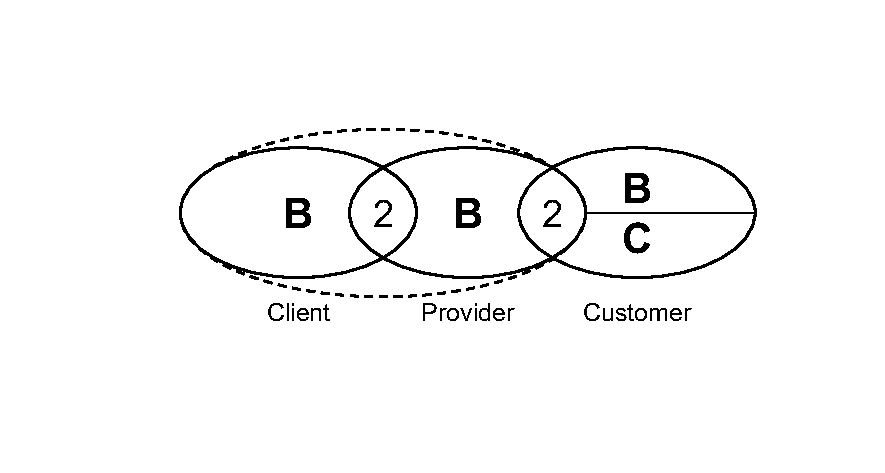
\includegraphics[width=.8\textwidth]{figures/bpochain.pdf}}
	\end{figure}

			
		\begin{itemize}
			\item IT as an enabler ok 
			\item offshore, nearshore, inshore - nur nennen und auf interessante Aspekte für case eingehen
			\item Model ? Matrix ? 
		\end{itemize}
	
		\subsubsection{Parent Company}
		%% irgendwie wiederkehrende Struktur bei Parent Company und Provider...
		Motivation for outsourcing of services is based on sound economic principles, as laid out in the section about the theory of the firm. From the previously described theories explaining outsourcing, especially the economic and strategic management view applies to justify outsourcing decisions. \citeauthor{bartell1998information} names improved business focus, mitigate risks, build sustainable competitive advantage, extend technical capabilities and free resources for core business purposes \citep{bartell1998information}. Cost reduction is not included in this list (even though it was a primary driver at first), as the experience has shown that 80\% of customer service outsourcing projects aimed for cost cutting are failing \footnote{\cf \url{http://www.gartner.com/newsroom/id/492113}}. 
		
		\todo{cost savings argument noch diskutieren, zahlen von schewe}
	
		\subsubsection{Outsourcing Provider}
		
		The business of an outsourcing provider is oriented towards clients. Outsourcing contracts are individually negotiated and can put the provider into different roles. While companies can use outsourcing as a means to drop off operative work and manage related processes by themselves, a closer relationship between provider and client facilitates more cooperation. Providers can become partners that take responsibilities collateral to their front-line business. 
		
		\cite{schewe2007} provide a framework about processes of an outsourcing provider, which is located in Appendix \ref{app:provproc}. It counts three main areas: Service management, delivery management and service delivery. Service management comprises \textit{client support} and \textit{help desk}, which are about the nurturing of the client relationship and providing help with respect to the provided services, respectively. Delivery management can be loosely compared to product development in a manufacturing business. It contains \textit{program management}, which handles the offered service portfolio and \textit{projects}, that develops and deploys new outsourcing engagements. The last area, service delivery, is about the outsourcing activity itself. Its components are finance, HR and Procurement / Logistics, as well as transaction processing. The latter refers to the creation of services, which is the main business, while the first three are supporting activities for service delivery. 
			
		A recent market overview segmented BPO-providers into five categories: \acrfull{HRO} specialists, customer care specialists, BPO multi's, IT multi's and document management providers \citep{hfs2016top}.  While the authors note that the split is subjective, it helps to get an overview about the market's composition, as shown in \Fig \ref{fig:bpomarket}. The notion of customer care is hardly seen in academics, as a search on sciencedirect unveils\footnote{1294 results for \enquote{customer service} in title, abstract or keywords in comparison to 58 for \enquote{customer care}}. It seems that customer care is used to emphasize activities that exceed narrow customer service provision. Here, the term \acrshort{CRM} is preferred to capture this extension, which is reasoned in the following.	
			
		\begin{figure}[caption={BPO market composition}, label={fig:bpomarket}]
			{	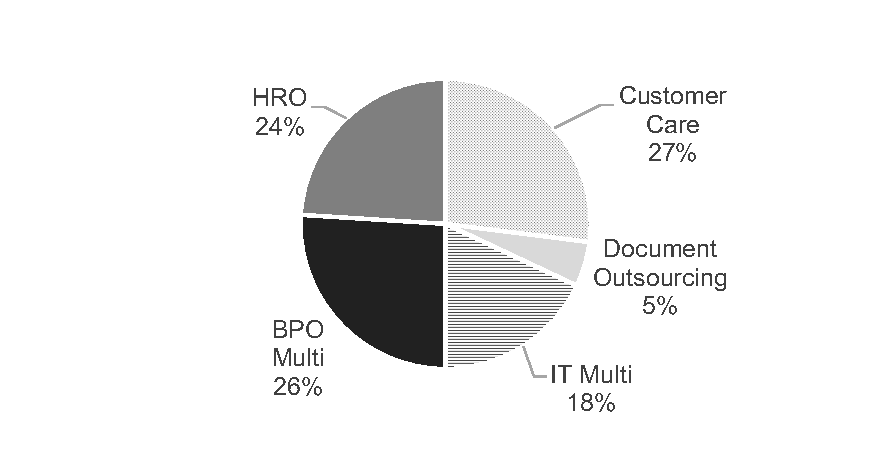
\includegraphics[width=.8\textwidth]{figures/bpomarket.pdf}}
		\end{figure}
	
		In terms of growth, customer care is expected to grow 4\%, which is one percent behind the highest growth rate of HR providers. 
	\todo{+market volume, geiler formulieren}
		%%%%%%%%%%
		\subsection{Customer Relationship Management}
		%%%%%%%%%
		\label{sec:crm}
		\enquote{A company's most precious asset is its relationship with its customers} is a quote of Theodore Levitt, Harvard Business School professor emeritus \citep{levitt1983}. Following this idea, marketing has undergone a shift from a brand- or product-centricity to a more customer-centered view \citep{Chen_2003}. An absence of sharp definitions has lead to a considerable confusion in academic literature about the term customer relationship management \citep{paynefrow2005}. 
		
		Essential terms surrounding CRM are marketing, relationship management and relationship marketing. Drawing on the taxonomy of \citep{hippnerwilde2011}, a visualization of the fundamental relationships is given in \Fig \ref{fig:crmcircles}. Under the umbrella of marketing, relationship management describes the active and systematic analysis, planning, design, selection and control of all business relationships in the sense of a holistic concept of systems, activities and goals \citep[\p{442}]{diller1995}. It has to be noted that not only relationship to customers, but also suppliers, communities, authorities, as well as internal relationship are enclosed by this term. Relationship marketing is a subset of relationship management and more strongly emphasizes customers as a target, but also comprises vertical relationships, i.e., relationships to suppliers. Within relationship marketing lies customer management or customer relationship management. Both terms are often used interchangeably  \citep{Leuer2011,ryals2001customer}. Conducting an analysis of publications \wrt the terms, \acrshort{CRM} is identified as the most used term (\cf \ref{app:mcoc}). Therefore, this thesis prefers the term customer relationship management.
		
		\begin{figure}[caption={CRM in the field of marketing}, label={fig:crmcirlces}]
			{	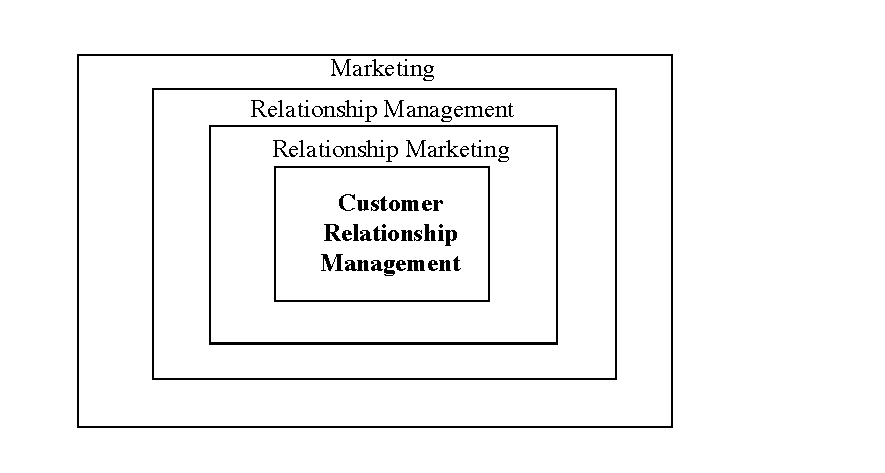
\includegraphics[width=.8\textwidth]{figures/crmcircles.pdf}}
		\end{figure}
	
		\citeauthor{Chen_2003} see a process, people and technology component in \acrshort{CRM} \citep{Chen_2003}. \cite{paynefrow2005} compile different standpoints and propose three views, that will be described in the following. As the name suggests, the building and sustaining of relationships to customers is always a defining characteristic of \acrshort{CRM}, but the importance of the technological component is varying. 
		
		Narrowly and tactically defined, \acrshort{CRM} refers to a technology solution and its implementation, which justifies the term's popularity in the technical field to create one view of the customer in the \acrshort{IS}. With an increased scope, \acrshort{CRM} can be seen as the implementation of an integrated series of customer-oriented technology solutions. Widely and strategically defined, \acrshort{CRM} can be seen as a holistic approach to managing customer relationships to maximize customer value, corporate profitability, and thus, shareholder value \citep{payne2004role}. This value is realized through the developed of a relationship, that is profitable and preferably long-term.  Customer service is seen as a part of \acrshort{CRM} \citep[\p{11}]{Helmke_2012}. It exists in order to create additional value before, during and after a purchase. 
	
		For this thesis, a customer is defined as an individual or business that has entered the process of buying a good or service from another business. Hence, the customer has a relation to the latter, that is of interest in CRM. This relationship can be strengthened by a plethora of marketing instruments that businesses use to bind the customer. These are initiated from the businesses and directed towards the customer. The reverse way, \ie, a customer reaching to the company by considering a product is also possible. 
		
			\begin{figure}[caption={CRM processes}, label={fig:crmprocessfr}]
			{	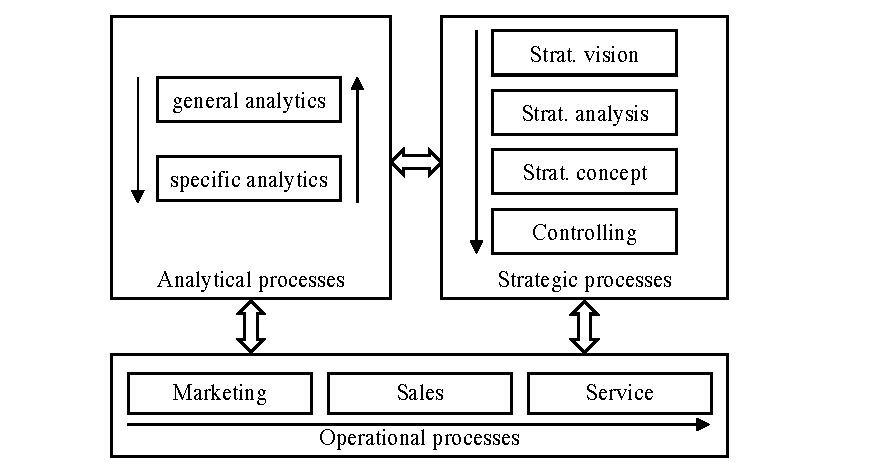
\includegraphics[width=.8\textwidth]{figures/crmprocessfr.pdf}
				
		\hspace{5.9cm}	SOURCE: adapted from \citep[\p{39}]{Helmke_2012}
				
			 }
		\end{figure}
	\todo{geil machen (boxen unten)}
		
		Processes in CRM can be divided into strategic, analytical and operative \citep{Neckel2005}. Strategic processes build up on an strategic analysis (for instance \acrfull{SWOT})) to derive goals of the CRM initiative and structures necessary to reach them. Operative processes describe execution loosely separated in marketing, sales and service processes. Analytical processes support both strategic and operative processes through data-driven insights either on a general level (\ie, customer segmentation) or bound to a specific activity (\ie, cross-selling). Operative processes are customer-facing processes and are of special interest in this thesis. 
		
		 For contact between the company and customer, two terms have emerged: (interaction) channels and customer touch points \citep{Leuer2011}. A channel is a medium that facilitates communication and seen from a company perspective, while a customer touch point is more specific and from the customer's view. A touch point shall be every moment of contact with the company from the customer's perspective \citep{Zomerdijk_2010}. Linking touch points together forms a customer journey. 
		 
		 A channel can be composed of platforms. Social media as a channel represents platforms like facebook, twitter or instagram. It will likely be a long-lasting medium in CRM, while a platform, may or may not withstand the test of time. Platform members can publicly communicate via posts, which are touch points between company and customer. 
		 However, it is noted that one can see platforms as channels in business, as the argument of platform popularity is of little interest in operations. This granularity stands in contrast to the intended applicability of this work, therefore a channel is  not seen as a platform here. 
		 In that sense, a channel is seen here as a more abstract type and a touch point an instance of a communication between company and customer. 
		
		Communication between the customer and company can be done through a number of channels which have grown in the past years. Integration of these channels is a central task of CRM and shows increasing complexity. \cite{paynefrow2005} propose six categories: (1) sales force, (2) outlets,\ie, stores and the alike, (3) telephony, (4) direct marketing,\ie, mail, radio, television, (5) e-commerce,\ie, e-mail and internet, (6) mobile-commerce (\ie, text messaging, mobile telephony). Applying the \acrfull{MECE}-rule, one faces problems with this definition. With the advent of smart phones, mutually exclusion of (3),(5) and (6) is hardly possible. In addition, social networks have become increasingly important for customer interaction. This necessitates another view, which conforms to today's channel landscape and is forearmed for new channels that might emerge in future. 
		
		This thesis takes a two-dimensional views on different interaction channels in CRM. Building on the framework by \citeauthor{paynefrow2005}, the digital component gets more emphasis, as it is of striking importance today. The matrix displayed in \ref{fig:channelmatrix} positions different channels with respect to their personal or universal way of communication, as well as their orientation towards IT. The aforementioned categories (1) sales force, (2) outlets and (4) direct marketing are located in the matrix with no further change of meaning to the primary literature. Especially in the digital sphere, a more diverse view on the remaining problematic categories is taken.
		
			\begin{figure}[caption={Channel matrix}, label={fig:channelmatrix}]
			{	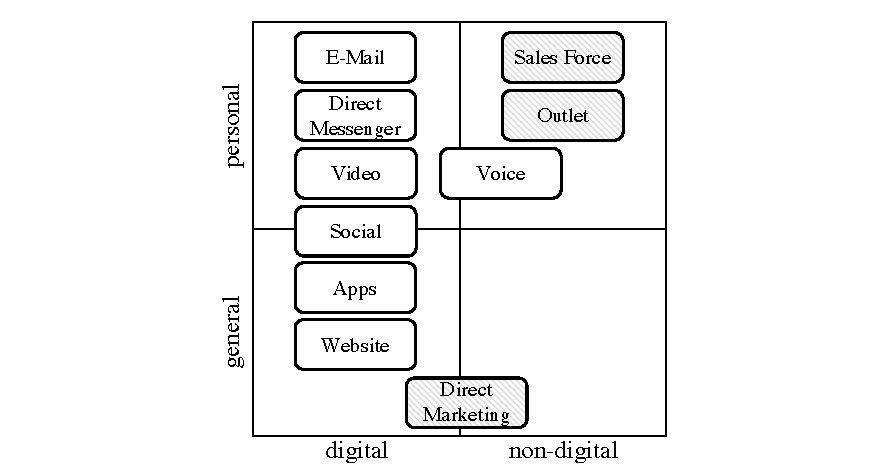
\includegraphics[width=.8\textwidth]{figures/channelmatrix.pdf}}
		\end{figure}
		
		Digital channels are characterized by the web as an underlying technology for communication. Non-digital channels on the other hands rely on real world interaction. In general, a shift towards digital channels is undeniable. For customers they are a convenient way of communication, as their devices enable them to do interact with less effort. A stop at a retail store is more effortful than a lookup of information on the company website. Nevertheless, non-digital channels will always be part of the channel portfolio, as complicated issues reason interaction with another human being face-to-face, especially in the B2B-sphere. 
		
		The customer-centric view underlines the shift to personal marketing activities \citep{peppers}. This is enabled by IT and the ever increasing amounts of data that is available and possibly attributable to a single consumer. While the more personal approach is standard practice in B2B-relationships, mass media direct marketing has been the only way to target private customers in the past decades through the use of radio or television. In a data-driven world personalized relationships with customers is an imperative to stay competitive. However, an anonymous way of retrieving information is also demanded, even though this way will likely increase the effort due to a less tailored presentation of information. This is contrary to the wish of integrating as much customer information as possible, to create a so called 360-degree view of the customer. Identification of customers for integration purposes is a key challenge there. 
		
		The two trends in the dimensions renders the personal / digital quadrant as an strategic priority.
		The identification of single customers is of paramount interest for a customer-centric view, which is only efficiently possible by information technology.  
		This again can be mapped back to the work of \citeauthor{paynefrow2005}: They name information management and multichannel integration as strategic processes. 
		
		Not every channel is used by every company, but companies tend to create multi-channel instead of single-channel strategies \citep{Frow_2007}. Coming from a pre-digital age, digital channels were integrated gradually and often in a heterogeneous information system landscape \citep{Chen_2003}. The following paragraphs shortly describe all channel categories that are not named  in  \cite{paynefrow2005}. A special focus is put on the role of customer service provision. 
		
		
		\subsubsection{Voice}
		
		Coming from traditional, non-digital telephony, voice is a very important service channel. While non-voice channels are said to overtake by the end of 2016, it is still accounting for half of the customer service volume on its own \citep{dimensiondata2016}. However, voice is becoming more and more digital for example through \acrfull{VOIP} technology, which is one reason for the renaming. Defining characteristic is the synchronous communication and interaction with a \acrfull{CSR}. A channel's popularity is reasoned by customer's expectation to explain their problem easily (35.2\%) and get a fast response (46.4\%) according to \citep{Agnischock2015}. Voice is well suited here, but is also a costly option for customer service through the one-to-one interaction. \acrshort{CSR}s are not able to process multiple calls simultaneously. Outsourcing call centers has therefore become a major application across industries (\todo{SRC und cost savings argument}) as low-wage countries like India offer significant savings. 
		
		Regarding data, the shift towards digital call processing enabled the tracking of numbers, efficient routing and conversation recording for instance. Identification of callers is often possible through the caller's phone number (if not suppressed), but a problem arises in outsourcing: When the client provides call routing systems and uses outsourcing as a means to process first level support for instance, the phone number might not reach the provider's systems. This renders a customer identification before start of the call impossible. Audio recordings also need to be automatically transformed into a processable format through sophisticated text-to-speech tools before using them for analytical purposes. Due to privacy reasons, these activities are restricted in many countries. 
		
		\subsubsection{E-Mail}
		
		By 2020, 50\% of the world's population is expected to have an email address \citep{radial2016}. In the developed world this number will be significantly higher. The convenience of electronic mail is the asynchronous communication from various devices, with attachments, at any time of the day and without the need to personally interact with the receiver. In customer service it is ranked second in terms of volume. 90.1\% of call centers support e-mail \citep{dimensiondata2016} today. %Traditional mail or fax is included in this category, as it is plays an subordinate role: 1.4\% of customers call it their preferred channel \citep{Agnischock2015}. It also offers significant obstacles for customers through its slowness, costs and effort of creation and sending. 
		
		As the message content is directly processable, analytical support plays an important role in routing mails. The sender can be identified by the address, that can not be suppressed. 
		\todo{+++}
		\subsubsection{Direct Messenger}
		The vast adoption of smart phones replaced the temporary very popular short messaging service (SMS) in a scratch.  While in 2012, traditional text messaging in Germany counted 162 million messages (the messenger whatsapp: 20 million), whatsapp overtook in 2013 and is now the goliath (667 million messages expected for 2015) in this business (39 million SMS are expected)\footnote{\cf \url{https://de.statista.com/statistik/daten/studie/3624/umfrage/entwicklung- der-anzahl-gesendeter-sms--mms-nachrichten-seit-1999/}}. The popularity stems from no character limit, no extra costs to their data plan and easy sharing of photos. Strong network effects tie users to the platform, while other players are existing in the market. In addition to this mobile app bound instances of messengers, many other platforms provide a direct messaging function, which is often called chat. Being a asynchronous channel from a technological perspective, it is de facto synchronous: customers expect a flowing conversation and hence a quick solution to their problems. Web sites of companies nowadays have a chat embedded to quickly solve issues that arise while browsing. An economic advantage for messengers in customer service is that an agent is able to process multiple chats in parallel, which is not possible in voice for example. In addition, automation technology enables artificial intelligence to participate in chats. Being fed and trained by a knowledge base, so called \textit{Chat Bots} are able to dynamically infer queries from customers that are transferred via chat messages. While complete control of bots is likely in future, support of human agents through analysis of chat input and recommending answer content contains less risk, as a human only gets decision support and still makes the decision. The reader is referred to \ref{sec:ss} for a discussion of self service technology in \acrshort{CRM}. 
		\todo{App abschnitt... oder einfach integrieren... ist in dem sinne auch kein channel, sondern wieder eine plattform, die informationen wie die website beinhaltet. }
		
		\subsubsection{Video}
		\todo{src}
		Video shares several characteristics with voice: It is synchronous, two human beings are involved and the communication is based on a common spoken language. In some sense, it is \textit{voice+}, as it adds the visual representation of communication partners, which is why one can argue that they will ultimately merge into one channel category. The reason for the split here is that voice has its roots in the non-digital world, while video is clearly a digital channel. In terms of adoption, voice is accepted and used across the technological, cultural and demographical sphere. This is not the case for video-based communication technology. While technological requirements (\ie mobile devices with front-cameras)  are given, it can be put into the early adopters group \wrt theory of diffusion of innovations \citep{rogers2010diffusion}. Consequently, the use in customer service is rarely seen. However, it offers advantages not possible via voice for example through the ability to perform legally binding identification or show objects of interest live during the conversation. These innovations are reasons to put it into place in customer service, as the customer knows of their necessity in the process. The technology acceptance model \citep{Adams_1992} helps to explain the obstacles: customers do not see the added value in revealing themselves visually in front of a stranger and also expect it to be more complicated than a normal phone call. 
		
		\subsubsection{Social}
		
		More than 40\% of Germans are members of a social network \footnote{\cf \url{https://www.statista.com/statistics/312918/social-network-penetration-in-germany/}}. The dominant player on this market in the western hemisphere is facebook. Characteristics of personal profiles and the ability to interact with ones network through public or private communication. The former is referred to as a post. With increasing private use, companies realized the potential in \acrshort{CRM} through these platforms. The ability to communicate \textit{with} the company on a public stage in the network is a novelty, which justifies its attractiveness for customers and companies. In customer service, it is often used as a channel for complaints, as publicly sharing ones grief puts more pressure on the company and hence benefits the chances of a customer to get a satisfying solution or compensation. The company needs to react quickly and well-considered to these inquiries, as the nature of social networks make it possible to generate a myriad of displeasing content by a single post (so called \textit{shit storms}). Furthermore, the answering agent represents the company as a single person in the post, which necessitates a review process. 
		
		The public posting also has implications on the ability to process customer inquiries. As personal or order related data should not be available on the network due to data privacy regulations, agents often have to switch to a private channel (\ie private messenger within the network or unrelated channel). Despite the use in customer service, companies also use social networks as a marketing channel. As typically all published content can be commented by users, there is no clear boundary between service and marketing activities. 
		
		
		\subsubsection{Website}
		
		A company's website is likely the first address a customer visits to satisfy his information needs. It can be a starting point for switching to another channel, \ie visiting the website for retrieving the service hotline number, or the channel that solves his problem. 15.1\% name it as their preferred contact channel \citep{Agnischock2015}. Often, a \acrfull{FAQ} section is provided to quickly answer questions in-demand. In addition to these sections, websites can offer a customer service area, that aims to solve customer's problem without personal interaction of a \acrshort{CSR}, which is called self service. The magnitude of these areas is varying largely by industry and company, as it is the companies own responsibility to design, implement and maintain it. A social network component can be seen in communities where customers help themselves. These brand communities \citep{Hsieh_2017} are typically moderated by \acrshort{CSR}s to ensure correctness of solutions. Elements of gamification give incentives to participate and follow the rules. This type of crowd-sourced knowledge is a substitute for customer service employees and therefore offers cost saving potential. 
		
		Furthermore, company websites may be platform for self service technology that actively processes queries against a knowledge base. Chat functionality can accompany the customer service area to give an medium to communicate issues in natural language, without the need to navigate through the website. 
			
		\subsubsection{App}
		Driven by ecosystems around smart phone operating systems (namely Android and iOS), small applications (apps) have emerged and enable diverse use cases for mobile devices. Companies publish their own apps to accompany products or services by additional information or functionality, which intensifies the relationship to the customer. Airlines for instance offer check-in over their app to improve customer experience and avoid queues and counters. Companies benefit from access to personal data, as the application needs to be installed. In terms of customer service, the app can be seen as a gateway to other channels, as a chat can be provided, web site content can be displayed or contact information for e-mail or calling can be shown. 
		
		\subsubsection{Non-Digital Channels}
		While digital channels continue to grow, other ways of contact exist. For customer service, the importance is diminishable if one counts voice as a digital channel : mail and fax account for 1.4\% across age groups \citep{Agnischock2015}, with the highest popularity among the elderly. These can be included in the e-mail channel, as their content can be digitized (\viz scanned). Brick and mortar stores, if available, amount for 28.5\% and are therefore very important. Narrowing the scope to \acrshort{ITES} leads to an exclusion of sales force or branches, as these are not outsourced. 
		
	
	\subsubsection{Self Services}
	\label{sec:ss}
		Self Service technologies enables customers to produce services without direct involvement of a service employee \citep{meuter2000self}. This automation is relying on information technology to enable its functionality. Early examples include ATMs or balance checks on cellphones, which underline the diversity of self-service channel opportunities. Today, the internet makes companies create comprehensive self-services, which are accessible through websites or apps. However, these examples convey that self service technologies cannot be seen as a channel, but as an additional component that enables service delivery standalone or combined with other services. 
		
		Standalone self services provide a solution to a customer's problem, \ie by providing the needed information in an \acrshort{FAQ} section (also called Self-Help \citep{meuter2000self}). Another possibility is the support in another service process, for example through call routing automation to the correct specialist in a call center. Here, the customer receives self-services by passing information to a technological interface, which in turn determines the contact, that solves his problem.  
		
		Reasons for self-service implementation are cost savings, due to less labor-intensity and scalability, as no employee needs to deal with the request. Customers can ignore service times and help themselves without the need to explain their issue to another person. \citeauthor{Blut_2016} provide a comprehensive study about technology acceptance in self service technologies \citep{Blut_2016}. 
		
	\subsubsection{Multi-Channel and Omni-Channel CRM}
		An explosion in touch points \citep{Lemon_2016}, especially in digital media, has lead to new developments in customer relationship management. Motivated by the availability of data across channels, its integration is a major challenge. Companies seek to make use of the data to enhance their customer relationships and improve customer experience across and within channels \citep{Frow_2007}. For this work, customer experience shall be defined as the internal and subjective response customers have to any contact (direct or indirect) with a company \citep{meyer2007customer}\footnote{\cf \cite{Lemon_2016} for a detailed discussion of customer experience and the customer journey }. In the last century \citeauthor{gilmore1998} claimed it will be the next \enquote{competitive battleground}, which now seems to come into reality. A recent study named customer experience the number one priority of executives in the next months \citep{acc2015ce}.
		
		\citeauthor{payne2004role} define five strategic\todo{wiederholung!} processes in \acrshort{CRM}, which include a multi-channel Integration process and an information management process \citep{payne2004role}. The former underlines the strategic role of integration from a customer experience perspective and the latter emphasizes the IT focus of CRM. 
		
		Two developments take place, multi-channel and omni-channel management. It is abstracting from the CRM case to include other domains, like retail. While multi-channel management is existing longer in the literature\footnote{For an overview of existing research see \citep{Neslin_2009}} and is now interpreted as the management of multiple channels to deliver high service quality in each of them, the notion of omni-channel management has recently emerged and seeks to deliver a seamless customer experience across channels. Omni-channel CRM originates in the domain of retail \citep{Brynjolfsson20131, rigby2011, Piotrowicz_2014} and envisioned shopping of goods across different sales channels (\ie online, store, telephone). This concept is now transferred from goods to the customer experience in its center, so that omni-channel management creates one view of a customer and thereby strengthens the relationship and increases its value. Measures like the customer lifetime value instead of value creation emphasize the long-term view of the customer \citep{Lemon_2016} and the need of CRM to run like a golden thread through different interactions of the customer. %This connection can be called customer journey. 
		
		Separating multi-channel from omni-channel is difficult, as the latter formed as an amplification of the latter. \cite{vorhoef2015retail} try a distinction shown in Table \ref{tab:mcoccomparison}, which is here masked from the retail domain. 
		
		\begin{table}[caption={Multi- and omni-channel comparison}, label={tab:mcoccomparison}]
			\centering
			\begin{tabular}{p{3cm}| p{5cm} |p{5cm}} 
				& \textbf{Multi-channel management}                                   & \textbf{Omni-channel management}                                                              \\ \hline
				\textit{Channel focus}                         & \textit{Interactive channels only}                                    & \textit{Interactive and mass-communication channels}                                                   \\ \hline
				\textit{Channes scope}                                 & \textit{Store, online website and direct marketing}                          & \textit{In addition mobile channels (\ie, smart phone, tablets, apps), social media}                   \\ \hline
				{Separation of channels}                           & Separate channels with no overlap                                  & Integrated channels providing seamless customer experiences                                   \\ \hline
				{Brand versus channel customer relationship focus} & Customer - channel focus                                            & Customer - channel - brand  focus                                                              \\ \hline
				{Channel management}                               & Per channel                                                         & Cross-channel                                                                                 \\ \hline
				{Objectives}                                       & Channel objectives (\ie sales per channel, experience per channel)& Cross channel objectives (\ie, overall customer experience, total sales over channels) \\
				\multicolumn{3}{r}{Adapted from \citep[\p{176}]{vorhoef2015retail}}
			\end{tabular}
		\end{table}
	 Aspects in channel focus and scope can be criticized in this juxtaposition. It is questionable that channels are excluded from multi-channel management, because in essence the distinction is seen in the relationship \textit{between} channels and not the channels themselves. The excluded channels from multi-channel management (\viz, mass communication) go back to the channel definition of \cite{Neslin2006}, which emphasizes interaction between customer and company. From this, \citeauthor{vorhoef2015retail} infer that solely two-way communication channels can be part of multi-channel management. The understanding in this work is different and makes no difference in possible channel focus and scope among omni- and multi-channel management. As \citeauthor{vorhoef2015retail} describe multi- and omni-channel as \enquote{phases}, they put mobile channels and social media as additions from multi- to omni-channel. This view might be reasoned in the publication time, because multi-channel publications in the early 2000s could not predict the impact of smart phones and tablets on marketing, as the more recent omni-channel publications. Appendix \ref{app:mcoc} holds an overview about publications over time regarding omni- and multi-channel management and proves the greater impact of multi-channel management over omni-channel management in the literature. 
	 
	 This work agrees with the view that omni-channel management puts in a holistic view and emphasizes communication with the brand across channels. The objectives of omni-channel management emphasize the overall, holistic customer experience, which forges a bridge to the \acrshort{CRM} domain. Adding the temporal dimension of the customer relationship, these experiences over different interactions (in separate, integrated channels) describe omni-channel \acrshort{CRM} as a means for a superior customer value creation. 
	 
	
		%%%%%%%%%%
		\subsection{Customer Relationship Management Business Process Outsourcing Providers}
		\label{sec:bpocrmis}
		%%%%%%%%%%
		Putting together the theory of business process outsourcing, customer relationship management and recent omni-channel approaches, this section underlines how these concepts work together in business. 
		
		From the process groups in \acrshort{CRM}, especially operational services are subject to outsourcing activities. Reasons for this lie in high intensity of manual work in customer service activities. While strategic or analytical processes are more connected to high skilled and differentiating activities for a company, customer service includes several tasks, that can be learned quickly. Outsourcing these makes use of (global) pay gaps and helps to realize cost savings. As the complexity of relationship management increases with the number of channels, companies find it harder to keep pace with their competitors. In addition, customers expect an individual and customized treatment, which justifies sophisticated techniques by companies, to know and accompany them on their customer journey. Consequently, BPO providers have expanded their tool set from being an extended work bench, to provide solutions for challenges in the other processes of CRM, namely strategy and analytics. 
		
		\citeauthor{Ramachandran2004} name two capabilities of outsourcing providers. On the one hand, they need to understand the client needs in the domain and business (\eg, CRM). This expertise is manifested in the understanding of the client's customer, as the relationship of the client to the customer is subject of the outsourcing engagement and is called the business development capability. Furthermore, the provider needs to have capabilities to execute the services efficiently. Economies of scale and scope have to realized by the provider to reach a competitive cost level and superior service, respectively, which are denoted as the operational capability.
		
		As visualized in  \ref{sec:frameworkbpo} \Fig \ref{fig:bpochain}, outsourcing provider and client can form one unit when an end customer is involved in the outsourced business. Customers need not be aware of the outsourcing contract and therefore the customer service provision should keep up this delusion. For instance, a \acrshort{CSR} in an outsourced setting will answer the phone on behalf of the client and does not leave any clues about being an employee of the outsourcing provider. As nowadays multiple channels are the norm, companies may outsource a subset of them, outsource all to one provider or cooperate with multiple providers (so called multi-vendor relationships)\todo{SRC}. Implications on providers arise when managing more than one channel, as the aforementioned multi- or omni-channel management approaches apply. This development requires more expertise from the provider and moves away from the extended work bench-analogy. The spanning of an outsourcing business across channels requires higher emphasis on information management and therefore the \acrshort{IS} landscape. Technological parameters can partly be set by the client, be it back-office systems or knowledge bases, as well as application systems that manage specific channels. Varying requirements and leeway make general statements about the provider's responsibilities vague. 
		
		Another dimension is the complexity of requests, which are outsourced. One typically differentiates in different tiers in a contact center\footnote{The term contact center or service center is preferred over call center, as nowadays more than calls are handled in these facilities.}, that order the complexity of inquiries. Tier 1 support solves the most basic queries and is typically the first personal contact in a service inquiry. Tier 2 support handles complex issues, where tier 1 support is not able to solve the problem. Consequently, tier 2 \acrshort{CSR}s need to be more skilled and trained than tier 1  \acrshort{CSR}s. This reasons why tier 1 customer service is the first outsourcing candidate (54\% tier 1 against 37\% tier 2 outsourcing \citep{deloitte2014outsourcing}): it is more labor intensive through its gate-keeping property and requires less training to be productive in the job. 
		
		In terms of \acrshort{IS} landscape, providers have to manage a plethora of customer service systems, as clients may bring in their own. In addition, they outsource single or multiple contact channels. Their own landscape may consist of a single system in the best case, but due to gradually introduction of digital channels, multiple systems are more likely. If new systems are put in place, clients may inherit the selection process, as the investment outlasts a typical outsourcing contract. Vendors on the market offer solutions for single or multiple channels and a provider selects the appropriate system for the client problem. Putting it into perspective across client businesses, the system landscape that the provider has to interact with can be described as highly heterogeneous, which is a reason why a centralized organization is hardly achievable. The client businesses need a sufficient amount of independence to meet client requirements. 
		\begin{itemize}
			\item ECIS Paper...

			\item hippner 680f
		\end{itemize}
	%%%%%%%%%%
	\section{Reference Modeling}
	\label{sec:03_refmod}
	%%%%%%%%%%
		%%%%%%%%%%
		\todo{intro}
Conceptual models are representations of an application domain used to capture the important features to be incorporated into a specific information system (Batani et al. 1992; Bodart et al. 2001). --37 vom brocke


		\subsection{Concept}
		
		\subsubsection{The Model as a construct}
		
		
		Reference Models can be seen as theory of information systems \citep{Schutte1998}. A model itself is defined as an \enquote{immaterial representation of an original for the purposes of a subject} \citep[\p{1}]{Becker2012Gom}. Based on the work of \cite{Stachowiak1973}, three characteristics of models are identified: mapping, reduction and pragmatism. Mapping describes the representation of natural or artificial originals, which can be models themselves. Reduction underlines the omission of certain elements of the original in a model. Pragmatism means that the selection of parts of the original is dependent on the intent of the model. Based on this notion, models of information systems (or information models in short) are explicit models that have information systems as subject matter. The purpose of modeling can be the constitution of application systems or the organization \citep[\p {59}]{Rosemann2012proc}. The latter is in focus here and encompasses among other aspects knowledge management, documentation of the organization and process management.Information modeling, the act of creating these models of \acrshort{IS} is a complex task, which is why reference models are a useful means to reduce this effort \citep{Becker2007} to create application models.
		 
			\subsubsection{Reference Models and Application Models}
			An information model can be specified on a certain company, which is here denoted as an application model. Reference models on the other hand are not firm-specific and as the name suggests provide guidance in a defined modeling scenario. There is no accepted definition of reference model in the literature. \citeauthor{thomas2006a} compiles various definitions for reference models \citep{thomas2006a}. \citeauthor{vom2006reusable} brings in the notion of reusable conceptual models, where conceptual models are the representations of an application domain used to capture the important features to be incorporated in a specific information system \citep[\p {584}]{vom2006reusable}, as the term reference model is predominantly used in the German literature. It is agreed that a reference or application model of German understanding is a conceptual model. However it is refrained to use the terms reference conceptual model and application conceptual model over \acrfull{RM} or \acrfull{AM} . As an conceptual model's purpose is the representation of features of an information system, it is an information model. 
			
			\citep{Schutte1998} puts \enquote{universal validity} and \enquote{recommending characteristics} as defining  for a reference model. Universal validity expresses that a reference model can only be valid for a class of companies, so that it can be used for creating application models. The recommending aspects states that a reference model should capture a wanted to-be state, which is in the modeler's intention. These two combined enable the wanted re-usability, which is planned by the modeler \citep[\p{36}]{brocke2003referenzmodellierung}. However, achieving a recommending characteristic is a subjective judgment and universal validity can always be achieved by shrinking down the target class of companies \citep{thomas2006a}. The other option, namely encompassing a large target class of companies to create \textit{one} reference model stands in contrast to practical use, as the creation of application models gets increasingly complicated the more general (and hence abstract and theoretical) \citep[\p{79}]{Schutte1998} the reference model is. Striking a balance between these trade-offs is known as the reference modeling dilemma \citep{delfmann2006adaptive}. 
		
			For this thesis, a reference model is defined as an information model with content that is reused in the construction of other application models. The relationship between a reference and application model is characterized by reuse of reference model components in application model construction (\cf \cite{Puster2015,brocke2003referenzmodellierung}). \todo{verbessern...}
			
			To capture the complexity in business, a data, organizational, functional or process perspective can be taken (\cf \ref{processorientation}). As only process models are subject matter in this thesis, the term process reference model is used interchangeably with reference model from here on. 
	\todo{vielleicht generisches RefModVariantenmanagement}
				  %delfmann: Variantenmanagement
				  
				  
				  
				  \begin{figure}[caption={Design Process of Reusable Conceptual Models}, label={fig:refmodconst}]
				  	{	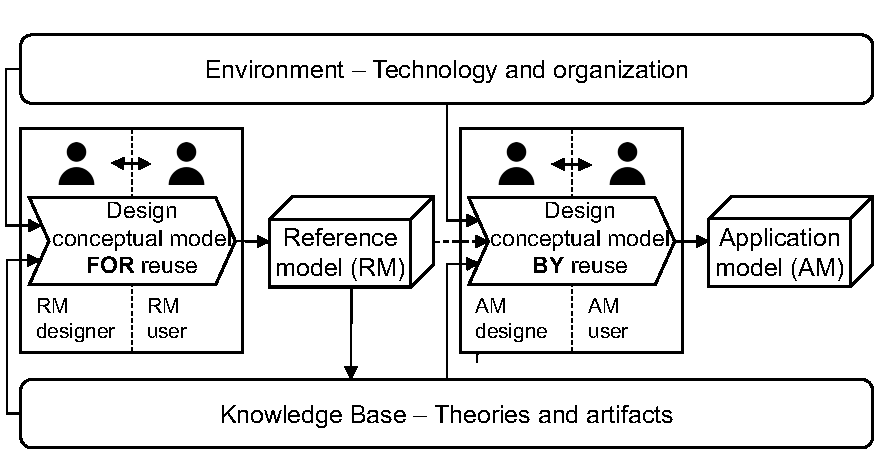
\includegraphics[width=.8\textwidth]{figures/refmodconst.pdf}}
				  	\hspace{6.2cm}	SOURCE:  adapted from \citep[\p{587}]{vom2006reusable}
				  \end{figure} 
				  
			%grafik aus refmod - enzyklopädie vom brocke
		A model is created by one or multiple subjects called designers and utilized by users \citep{becker2004handelsinformationssysteme}. Model designers in context of reference modeling responsible for creating the \acrshort{RM} itself. Their intention is to design \textit{for} reuse, \ie creating an artifact that is to be reused. The other involved stakeholder in this modeling process is the reference model user which collaborates with the designer and defines requirements for use. This first process is visualized in the left chevron in \Fig \ref{fig:refmodconst} and takes input from the knowledge base as well as the environment. The output is the  \acrshort{RM} which itself contributes to the knowledge base as an artifact. 
		
		The right chevron is similarly structured \wrt the stakeholders, but designs an application model on base of the now existing \acrshort{RM} which can be labeled as design \textit{by} reuse. Akin to the reference model designer, the application model designer takes requirements from the application model user. By doing this, the  \acrshort{AM} can represent characteristics of the application environment (\ie one organization), while still being conformable to the reference model. 
		
		\subsection{Construction}
		A construction of an \acrshort{AM} on basis of a \acrshort{RM} requires the construction of the latter beforehand. 
		\Fig \ref{fig:refmodconst} lists the knowledge base (theories and artifacts) and the environment (technology and organization) as inputs for reference modeling. For knowledge acquisition, one can differentiate in an inductive and deductive approach \citep{thomas2006mang}. Inductive conclusions  might stem from the organizational settings that are observed or existing \acrshort{AM}s of organizations in the domain. Deduction is employed when drawing on existing theories from the knowledge base. Loosely, these two approaches refer to the two inputs for design \textit{for} reuse in \Fig \ref{fig:refmodconst}. 
		
		The reader is referenced to \cite{Fettke2014meth} for an overview about different construction techniques. These show conformance with the design science approach \citep[\p{10}]{Puster2015} which is taken here. 
		
		
		\subsubsection{Selected Reference Models}
		
		As mentioned, a reference model is suited to fit requirements of a certain domain. The purpose of this section is to briefly present two different reference models that are used in practice: The \acrfull{SCOR} Model and the Retail-H. Both show a layer structure to manage complexity and both encompass a process reference model. 
		
		\acrshort{SCOR} allows modeling of supply chains. It is a process reference model with three detail layers. It was developed in 1996 and is now maintained by the Association for Operations Management \citep{APICS2015}. On the highest level, typically called regulatory framework, \acrshort{SCOR}  is based on six distinct management processes: Plan, Source, Make, Deliver, Return and Enable. While the regulatory framework assists in defining scope, the second configures the type of supply chain (Make-to-Order, Build-to-Order, Engineer-to-Order). On the thirds level these are decomposed into generic process steps (e.g., issue product). Even more detailed processes are considered company specific and therefore no part of the model. Furthermore, performance metrics are also defined on each level. 

		\begin{figure}[caption={SCOR Model}, label={fig:scor}]
		{	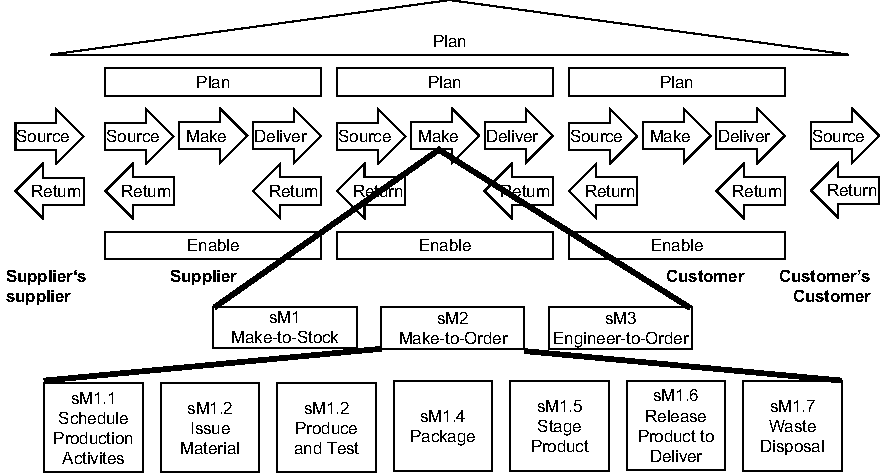
\includegraphics[width=.8\textwidth]{figures/scor.pdf}}
			\hspace{6.2cm}	SOURCE: ...
		\end{figure}
	

		In the domain of retail, the Retail-H is a reference model that includes process, function and data models. Developed by \cite{becker2004handelsinformationssysteme}, it has been adapted to suit special segments of the domain\footnote{for instance eCommerce, Central Clearance or Central Settlement \citep{Puster2015}}. 
		It is structured with four layers of detail: the regulatory framework, main processes, detail processes and process building blocks, as an application of icebricks as a process modeling language. The core of the regulatory framework is made up of three parts that form the H (a connection to the German word for retail: \enquote{Handel}). While the left part of the H describes the supply side, the right covers the distribution side. Both are connected through logistics. All of these core processes are business processes, the roof and foundation consist of support processes thereby making use of the framework reference design as proposed in \cite{Meise2001} while simultaneously capturing domain-specific aspects in the set-up of the framework.  
		
		\begin{figure}[caption={Retail-H}, label={fig:retailh}]
			{	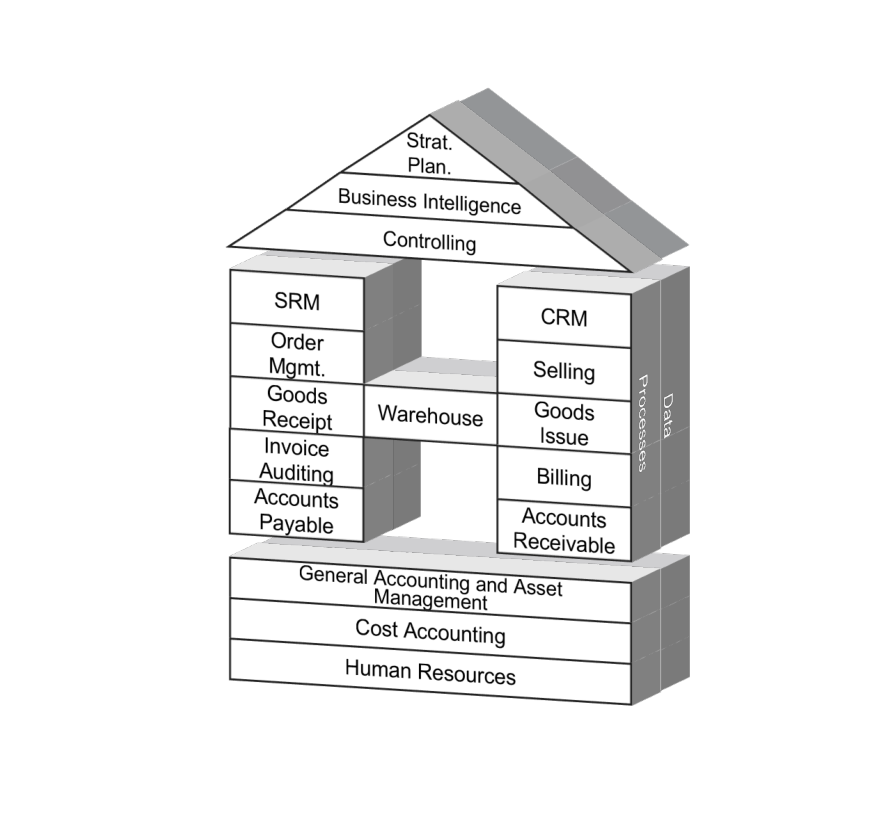
\includegraphics[width=.6\textwidth]{figures/retailh.pdf}}
			\hspace{6.2cm}	SOURCE:  ....
		\end{figure}
		

		%%%%%%%%%%

		%%%%%%%%%%
		\subsection{Benefits}
		
		\citeauthor{becker2004handelsinformationssysteme} name benefits of reference models in combination with an explorative study \citep[\pp{75}]{Schutte1998}. Similar to \cite{vom2006reusable}, they differentiate in model designers and users. Reflecting on \Fig \ref{fig:refmodconst}, actors in the left process are subject in this section. Taking the view of the two parties, the following benefits are named:
		
		\begin{itemize}
			\item Designers
			\subitem Monetization through application and configuration
			\subitem Obtaining domain knowledge
			\item Users
			\subitem Cost reduction
			\subitem Risk reduction
			\subitem Documentation
			\subitem Analysis
			\subitem Exchange of information  
		\end{itemize} 
	
		Designers of \acrshort{RM} are a research institutions or businesses. This distinction is not mutually exclusive,  but helps to conclude the two main benefits. While the economic principles encourage the monetization through the use of the \textit{product} reference model, the scientific world strives for cognition in the domain. It is noted, that the practical use of a reference model to form an application model is seen as hardly possible without additional consultative services in application model design \citep{Schutte1998}.
	
		The user side puts emphasis on cost reduction aspects \todo{schütte?}. This stems from the avoidance of modeling from scratch which creates quality gains and time savings. Related to this, risk reduction refers to less modeling mistakes as the application model builds on a solid foundation. Through a more structured approach of information modeling an improved documentation can be achieved. The analysis and identification of weak spots is especially important in process reference models \citep[\p{81}]{becker2004handelsinformationssysteme}. Finally, the exchange of information inside the company benefits from a common base for discussion. \cite{glossar nicht wirklich zwingend drin...}A glossary for an unified terminology additionally supports communication inside the company, as well as with other reference model using companies. It can be summarized as \textit{best practice sharing}. A feedback loop from users to designers also facilitates further development and adjustment of existing \acrshort{RM} to new circumstances in the domain. \todo{vombrocke checken!}
		
		%%%%%%%%%%
		%%%%%%%%%%
		\subsection{icebricks as a Process Modeling Language}
		
	 A language is a system of signs and rules to their use \citep[\p{11}]{holten1999}. Fundamental is the ability to represent and communicate information through it \citep[\p{64}]{brocke2003referenzmodellierung}. While reference models are formulated in various languages, several options may arise. There are reference models like \acrshort{SCOR}, which avoid the use of a defined modeling language to ensure wide industry adoption through not interfering with used modeling languages. However, this necessitates an increased complexity in adoption, as an application within a company requires the translation into a sound process modeling language. While the framework level does not need to comply to a formalized language, more detailed layers of the reference model without clearly defined syntactical guidance increase the risk of misunderstanding among users.
	 This reasons the choice of using a defined process modeling language for this undertaking.
	 
	 The next step is to decide what language to use. Traditional modeling languages like the \acrfull{EPC} or \acrfull{BPMN} show similarities. Being syntactical languages, they offer large degrees of freedom in usage. What might look like an advantage at first sight, turns out to be disadvantageous. As process management approaches have increased number and variety of model designers and users enormously, more and more non-experts get in contact with process models and thus create models of less quality. \todo{SRC} The definition of modeling conventions becomes necessary to help the modeler to conform certain standards. A way to confront this challenge are the \acrfull{GOM} \citep{BeckerGOM2012}, which are an analogy to the \acrfull{GAAP}. However, conforming to these guidelines will lead to increased resource requirements in these undertakings. Semantic process modeling languages avoid this by enforcing additional rules that models have to follow. icebricks \citep{becker2015icebricks} is one example that realizes this concept and has been used for reference modeling. In addition to syntactical correctness, \ie conforming to an existing language's meta model, other aspects are also considered which would otherwise be taken care of by combining \acrshort{GOM} and syntactical languages. Because the additional check for guideline compliance is unnecessary in semantic languages, they are more efficient. After a short summary of the language,  the \acrshort{GOM} are described and it is argued why icebricks conforms to the aspects. 
	 
	 icebricks has a four layer architecture, which consists of four layers of abstraction: (1) process framework, (2) main process, (3) detail process and (4) process building blocks. Each lower layer is an element of the higher layer, i.e. an element on the framework layer is a main process. Each part of a main process is a detail process and so on. A glossary ensures unambiguous terminology and meaning of processes. Variants are integrated in the layer concept, so that every main or detail process can have different variants to model different peculiarities within a process. One example can be the three variants make-to-stock, make-to-order or make-to-engineer as variants of a production process. icebricks uses undirected graphs, which enables non-sequential flow of activities. 
	 
	 
	 \subsubsection{Correctness}
	 Correctness can be seen from a semantical and syntactical point of view. The latter can be assured when the model conforms to a meta-model of the language, which is shown in \ref{fig:icebricksmetamodel}. On the other hand, semantical correctness refers to the correct display of content inside the model. This correctness is hard to prove, but can be supported by a clear and simple structure that minimizes misunderstanding (which negatively impacts semantical correctness). While the other named languages tend to generate very complex models, the strict four layer structure of icebricks limits model complexity. 
	 
	 	 \begin{figure}[caption={icebricks meta model}, label={fig:icebricksmetamodel}]
	 	{	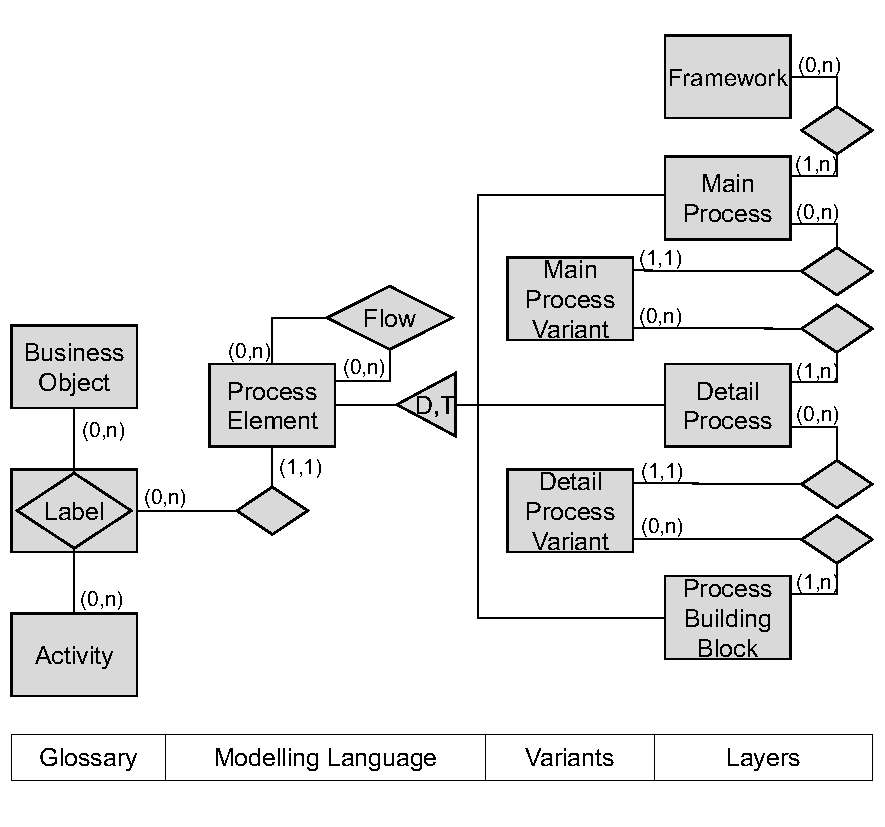
\includegraphics[width=.8\textwidth]{figures/icebricksmetamodel.pdf}}
	 	\hspace{6.2cm}	SOURCE:  adapted from \citep[\p{75}]{Puster2015}
	 \end{figure} 
 
	 \subsubsection{Relevance}
	 Relevance refers to the depiction of elements inside the model, which are necessary for the modeling purpose. This causes two boundaries: On the one hand, no element should be included in the model that has no connection to the real world. On the other hand, no aspect of the real world should be part of the model, which does not comply with the modeling purpose. Again, a simple structure of processes helps to guide the modeling procedure. 
	 
	  \subsubsection{Economic efficiency}
	 Syntactical languages are more error prone than semantical languages, because defects occur a posteriori, \ie, after modeling. As a semantical language ensures more guidance and strictness to its modeler, less errors exist in the model because they are identified during model creation. This reduces corrections on the outcome, which benefits the economic goal of successfully creating a model for the intended purpose with minimal effort (efficiency). In addition, icebricks as a reference modeling language has the ability to translate into other languages, because it only uses activities and control flow on every level. This enables a more efficient application of the reference model in companies and positively effects learning and use the language \citep{Muehlen}. 
	 
	 \subsubsection{Clarity}
	 Clarity aims at a clear structure within a model and a simple navigation through different process models. The four layer approach, variant modeling and limited use of branches addresses a clear and consistent structure in an icebricks process model. Furthermore, the glossary ensures a labeling of processes, that conforms to the proposed verb + object construct \citep{7pmg} and tackles the problem of naming conflicts.
	 
	 \subsubsection{Comparability} 
	 With respect to different modeling languages, comparability describes the transfer of content inside a model in language A to another language B without sacrificing information. icebricks was designed to provide this ability, as the application of a reference model in multiple companies consequently leads to contact with different process modeling languages. The transfer to \acrshort{EPC},\acrshort{BPMN} can be performed lossless. \todo{püster?}
	 
	 \subsubsection{Systematic Design}
	 The scope of reference models necessitates different layers of detail to manage complexity. Consistence between different layers is a challenge when separate models are built for each layer. By applying a layer structure, variant modeling and the use of a glossary, icebricks guides the modeler during model creation to create well-structured models in the first place. 

	
